\chapter{Revue de littérature sur la tâche d'annotation en intelligence artificielle}
\label{chapter:2-REVUE-DE-LITTERATURE}
	\todo[inline]{CHAPITRE: TITRE À TROUVER: "\textit{(Revue de littérature)}"}
	
	% RÉSUMÉ DES ÉPISODES PRÉCÉDENTS: 
	\todo[inline]{CHAPITRE: INTRODUCTION À RÉDIGER}
	
	% ANNONCE DU BUT DU CHAPITRE: 
	\todo[inline]{CHAPITRE: INTRODUCTION À RÉDIGER}
	
	% TABLE DES MATIÈRES DU CHAPITRE
    \minitoc
	
    %%%%%--------------------------------------------------------------------
    %%%%% Section 2.1:
    %%%%%--------------------------------------------------------------------
    \section{Présentation théorique de l'annotation}
	\label{section:2.1-PRESENTATION-ANNOTATION}
	
		% Introduction: donner une définition de ce qu'est l'annotation.
		Tout d'abord, définissons ce que nous appelons « \texttt{annotation} » et donnons quelques exemples pour comprendre les enjeux qui y sont associés.
		
		
		%%%
		%%% Subsection 2.1.1: Définition et objectifs de l'annotation de données.
		%%%
		\subsection{Définition et objectifs de l'annotation de données}
		\label{section:2.1.1-PRESENTATION-ANNOTATION-DEFINITION}
			
			%%% Corpus.
			\paragraph{Qu'est qu'un « \texttt{corpus} » ?}
			% Définition de "corpus".
			Certains phénomènes peuvent être difficiles à cerner à cause de leur nature complexe : c'est le cas par exemple avec le langage humain, la diversité de la faune et de la flore, les variétés d'un répertoire musical ou cinématographique, ...
			Pour nous aider à capturer ces phénomène et à mieux les comprendre, il est possible de les décrire par l'exemple en recueillant des textes, des images, des sons, des vidéos, ou tout autres relevés d'informations : nous utilisons alors le terme « \textbf{corpus} » pour désigner cet ensemble de données.
			Par aspect pratique, il est généralement stocké dans un format exploitable par une machine (\textit{fichier texte, base de données, ...}).
			
			% Carcatéristique importante : la représentativité !
			Un corpus n'est qu'un échantillon de taille finie d'un phénomène pouvant être infini ou indénombrable.
			Il est donc d'usage de valoriser un corpus s'il est « \textbf{représentatif} » du phénomène qu'il décrit, c'est-à-dire s'il capture bien le large panel de variations que peuvent prendre les données (\cite{biber:1993:representativeness-corpus-design}).
			
			% References.
			\begin{leftBarInformation}
				Si vous voulez mieux comprendre cette notion de corpus, vous pouvez vous référer à \cite{sinclair:2004:corpus-text-basic} issu du livre \textit{Developing Linguistic Corpora} (\cite{wynne:2004:developing-linguistic-corpora}).
			\end{leftBarInformation}
			
			%%% Annotation.
			\paragraph{Qu'est que l'« \texttt{annotation} » ?}
			% Définition de "annotation".
			Les données d'un corpus manquent parfois d'information pour bien cerner un phénomène, il est alors nécessaire de faire intervenir un humain pour introduire des connaissances supplémentaires qui ne sont pas explicitement présentes dans les données.
			Nous appelons alors « \texttt{annotation} » cette tâche consistant à décrire les données d'un corpus.
			On distingue alors les données dites « \textbf{brutes} » des données dites « \textbf{annotées} » en fonction de l'absence ou la présence d'un complément d'informations.
			
			% Valeurs associées: valeur ajoutée, information d'interprétation.
			Dans la littérature, \cite{garside-etal:1997:corpus-annotation-linguistic} présente l'annotation comme la tâche permettant de donner une « \textbf{valeur ajoutée} » aux données ; de son côté, \cite{leech:2004:adding-linguistic-annotation} précise que l'annotation permet ainsi d'interpréter les données pour mieux comprendre un phénomène, mais aussi d'entraîner un modèle d'apprentissage automatique pour le prédire voire le reproduire.
		
		
		%%%
		%%% Subsection 2.1.2: Exemples de tâches d'annotations.
		%%%
		\subsection{Exemples de tâches d'annotations}
		\label{section:2.1.2-PRESENTATION-ANNOTATION-EXEMPLES}
			
			% Transition: définitions assez généralistes car champ d'application très vaste.
			Les définitions données dans la section précédente sont volontairement abstraites car il est difficile de dépeindre la vaste diversité d'applications nécessitant une tâche d'annotation.
			En effet, il y a une telle multiplicité de types de données (\textit{données tabulaires, textuelles, visuelles, auditives, ...}) et de cas d'usages (\textit{prédiction d'une valeur numérique (tâche de régression), prédiction d'une catégorie (tâche de classification), détection d'objets (tâche d'extraction), création de nouvelles données (tâche de génération), ... }) qu'une unique définition ne peut être que purement théorique.
			%Ainsi, on constate dans la littérature que les présentations de la tâche d'annotation (comme les ouvrages cités plus haut) partent d'une définition générale pour rapidement l'appliquer à une activité bien précise (\textit{l'étiquettage grammaticale dans \cite{garside-etal:1997:corpus-annotation-linguistic} par exemple}).
			
			% Annonce: prendre des exemples sur l'univers de la bande dessinée.
			Ainsi, nous pensons qu'il est préférable de compléter ces définitions par quelques exemples concrets : nous pourrons ainsi mieux dresser le portait d'une tâche d'annotation, avec ses intérêts et ses complications.
			Pour cela, nous allons prendre le thème de la bande dessinée et de ses dérivés, et explorer ensemble les différentes cas d'usage qui pourraient intéresser un auteur, un libraire ou un lecteur.
			Pour faciliter la lecture, nous regrouperons ces applications en fonction du type de données qu'elles manipulent.
			
			%%% A. Annotation de données structurées: régression linéaire d'un prix.
			\paragraph{Annotation de données structurées.}
			
				% Cas d'usage: évaluer le juste prix.
				Les acheteurs et les vendeurs de bandes dessinées s'interrogent forcément sur le juste prix de l'oeuvre qu'ils veulent acquérir ou céder.
				Répondre à cette question avec précision nécessite diverses informations, à la fois sur l'oeuvre (comme son identification ou l'avis de ses lecteurs), sur le document en tant que tel (comme son état de conservation), mais aussi sur le prestige de son édition (éditions originales ou de collection).
				Sans un regard d'expert, il est possible de trouver certaines oeuvres rares vendues pour presque rien sur le marché d'occasion, ou à l'inverse voir certaines \texttt{BD} achetées à prix d'or alors que le document est en piteux état.
				
				% Entrainer un modèle: régression linéaire.
				Afin d'aiguiller les acquéreurs, il est possible d’utiliser un modèle de \textbf{régression linéaire}\footnote{Pour plus de détails sur la régression linéaire: voir la revue de \cite{maalouf:2011:logistic-regression-data} et voir \cite{zdaniuk:2014:ordinary-leastsquares-ols} pour un exemple basé sur la méthode des moindres carrés.} permettant de prédire le prix d'une \texttt{BD} à partir des différentes métadonnées discutées ci-dessus.
				Mais pour entraîner un tel modèle, une base d'exemples reliant une transaction à son prix de vente est nécessaire.
				La tâche d'annotation peut alors consister à renseigner pour chaque transaction :
				\begin{itemize}
					\item l'identification objective d'après des sources officielles (titre, auteur, édition, ... ),
					\item l'état du document grâce à un regard d'expert (l'état peut par exemple être défini par une variable catégorielle dont les valeur seraient "\texttt{Mauvais état}", "\texttt{Bon état}", "\texttt{Très bon état})", "\texttt{Neuf}") ;
					\item le prix du document, estimé ou réel (défini par une variable numérique).
				\end{itemize}
				
				% Citation de l'exemple.
				Un exemple de résultat d'annotation de ces données structurées sont disponibles dans la \textsc{Table~\ref{table:2.1.2-PRESENTATION-ANNOTATION-EXEMPLES-TABLE-VENTE-BD}}.
				%
				\begin{leftBarExamples}
					\begin{table}[H]  % keep [H] to be in the tcolorbox.
						\begin{center}
						\def\arraystretch{0.8}  % interligne
						\begin{tabular}{|c|l|c|c|c|r|}
						
						\hline
						% ENTETE DU TABLEAU
						Collection
							& N°: Titre
							& Édition
							& Note
							& État
							& Prix (€)
							\tabularnewline
							\hline
						% BD1.
						Lucky Luke
							& $01$: La mine d'or de Dick Digger
							& $1949$
							& $3.2/5$
							& Très bon
							& $5~000,00$
							\tabularnewline
							\hline
						% BD2.
						Lucky Luke
							& $12$: Les cousins Dalton
							& $1958$
							& $4.3/5$
							& Bon
							& $40,00$
							\tabularnewline
							\hline
						% BD3.
						Lucky Luke
							& $12$: Les cousins Dalton
							& $1962$
							& $4.3/5$
							& Très bon
							& $65,00$
							\tabularnewline
							\hline
						% BD4.
						Lucky Luke
							& $12$: Les cousins Dalton
							& $1985$
							& $4.3/5$
							& Très bon
							& $6,00$
							\tabularnewline
							\hline
						% BD5.
						Lucky Luke
							& $15$: L'évasion des Dalton
							& $1960$
							& $4.1/5$
							& Mauvais
							& $3,00$
							\tabularnewline
							\hline
						% ...
						\multicolumn{6}{|c|}{ \shortstack{ ... } }
							\tabularnewline
							\hline
					
						\end{tabular}
						\end{center}
						\caption{
							Exemple d'annotation du prix de vente de bandes dessinées en fonction de leur édition, de la note de leur lecteurs et de leur état (source: \url{https://www.bedetheque.com/serie-213-BD-Lucky-Luke.html}).
						}
						\label{table:2.1.2-PRESENTATION-ANNOTATION-EXEMPLES-TABLE-VENTE-BD}
					\end{table}
				\end{leftBarExamples}
				
				% Autres cas d'usage.
				\todo[inline]{autre cas d'usage: classification ? statistiques ?}
			
			
			%%% B. Annotation d' images: classification de document, catégorisation, détection d'objets, ...
			\paragraph{Annotation d'images.}
				
				% Cas d'usage: identifier une bande dessinée
				Identifier une bande dessinée n'est pas toujours facile, et recopier l'ensemble des informations l'identifiant peut prendre du temps.
				Les libraires ou les collectionneurs désirant faire l'inventaire des oeuvres en leur possession peuvent ainsi y passer de nombreuses heures, avec le risque de faire des erreurs lors de l'inscription des \texttt{BD} dans leur registre.
				
				% Entrainer un modèle: extraction de caractères.
				Afin d'aider les collectionneurs, il est possible d'utiliser un modèle de \textbf{reconnaissance optique des caractères} (\texttt{OCR})\footnote{Pour plus de détails sur l'\texttt{OCR}: voir la revue de \cite{berchmans-kumar:2014:optical-character-recognition} ou de \cite{awel-abidi:2019:review-optical-character}.} pour identifier les informations importantes présentes sur les couvertures des oeuvres à identifier.
				Mais pour entraîner un tel modèle, une base d'exemples reliant des captures de la page de couverture, la position des informations sur ces captures ainsi que la valeur de ces informations est nécessaire.
				La tâche d'annotation peut alors consister à renseigner pour chaque couverture de \texttt{BD} :
				\begin{itemize}
					\item la position des informations en l'entourant sur l'image (avec un rectangle par exemple) ;
					\item la valeur écrite à chaque information positionnée.
				\end{itemize}
				
				% Citation de l'exemple.
				Un exemple d'annotation de textes dans un image est disponible dans la \textsc{Figure~\ref{figure:2.1.2-PRESENTATION-ANNOTATION-EXEMPLES-IMAGE-OCR}}.
				%
				\begin{leftBarExamples}
					\begin{figure}[H]
						\centering
						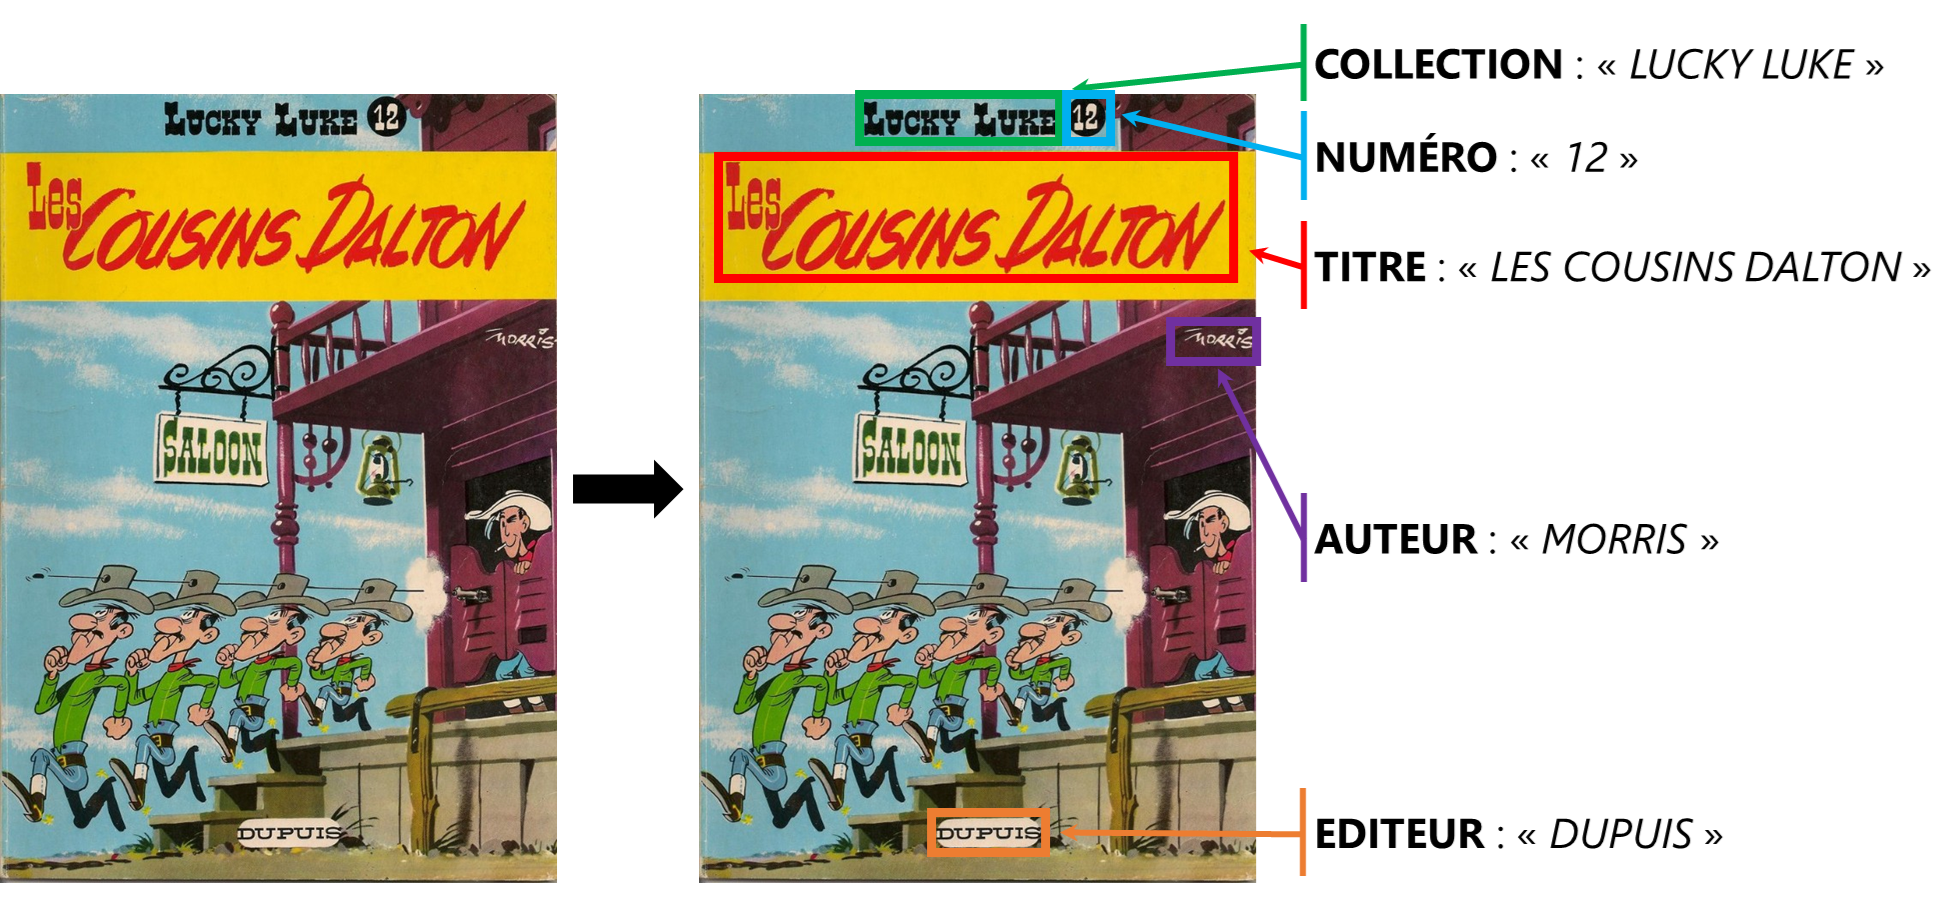
\includegraphics[width=0.95\textwidth]{figures/etatdelart-morris-1958-lucky-luke-12}
						\caption{
							Exemple d'annotation de textes présents sur la couverture d'une bande dessinée \texttt{BD} (ici: \cite{morris-goscinny:1958:cousins-dalton}).
						}
						\label{figure:2.1.2-PRESENTATION-ANNOTATION-EXEMPLES-IMAGE-OCR}
					\end{figure}
				\end{leftBarExamples}
				
				% Autres cas d'usage.
				\todo[inline]{autre cas d'usage: identification par une description ? classification de l'état ?}
			
			% C. Annotation textes: catégorisation, détection de sentiment, extraction d'entités nommées, ...
			\paragraph{Annotation de textes.}
				\todo[inline]{SECTION: À RÉDIGER}
			
				% Cas d'usage: 
				% Entrainer un modèle:
				% Citation de l'exemple.
				
				\begin{leftBarExamples}
					Annotation d'une classification de textes suivant leur langue.
					\begin{center}
					\begin{tabular}{ c l }
						« \textit{
							Les cousins Dalton ont dévalisé la diligence.
						} » & $\implies$ \textcolor{colorSilverLakeBlue}{\texttt{Français}} \\
						« \textit{
							The Dalton cousins robbed the stagecoach.
						} » & $\implies$ \textcolor{colorDarkPastelGreen}{\texttt{Anglais}} \\
						« \textit{
							Die Dalton-Cousins haben die Postkutsche ausgeraubt.
						} » & $\implies$ \textcolor{colorDarkPastelRed}{\texttt{Allemand}}
					\end{tabular}
					\end{center}
				\end{leftBarExamples}
				
				\begin{leftBarExamples}
					Annotation d'entités nommés dans un texte.
					\begin{quote}
						« \textit{
							$\textbf{\text{Lucky Luke}}_{\textcolor{colorDarkPastelRed}{\texttt{(personnage)}}}$, le $\textbf{\text{cow-boy}}_{\textcolor{colorDarkPastelPurple}{\texttt{(métier)}}}$ solitaire, a attrapé les $\textbf{\text{Dalton}}_{\textcolor{colorDarkPastelRed}{\texttt{(personnage)}}}$ à $\textbf{\text{Coyote Gulch}}_{\textcolor{colorCarrotOrange}{\texttt{(lieu)}}}$ et a touché $\textbf{\text{50.000\$}}_{\textcolor{colorSilverLakeBlue}{\texttt{(argent)}}}$ en les livrant au $\textbf{\text{pénitencier}}_{\textcolor{colorCarrotOrange}{\texttt{(lieu)}}}$. Ils se sont évadés le $\textbf{\text{jeudi suivant}}_{\textcolor{colorDarkPastelGreen}{\texttt{(date)}}}$.
						} »
					\end{quote}
				\end{leftBarExamples}
				
				\begin{leftBarExamples}
					Annotation des étiquettes grammaticales dans un texte.
					\begin{quote}
						« \textit{
							$\text{Les}_{\textcolor{colorDarkPastelPurple}{\texttt{(DET)}}}$
							$\text{dangereux}_{\textcolor{colorMinionYellow}{\texttt{(ADJ)}}}$
							$\text{Dalton}_{\textcolor{colorDarkPastelRed}{\texttt{(PROPN)}}}$
							$\text{se}_{\textcolor{colorCarrotOrange}{\texttt{(PRON)}}}$
							$\text{sont}_{\textcolor{colorDarkPastelGreen}{\texttt{(AUX)}}}$
							$\text{encore}_{\textcolor{colorSilverLakeBlue}{\texttt{(ADV)}}}$
							$\text{évadés}_{\textcolor{colorDarkPastelGreen}{\texttt{(VERB)}}}$
							$\text{de}_{\textcolor{colorDimGray}{\texttt{(ADP)}}}$
							$\text{prison}_{\textcolor{colorDarkPastelRed}{\texttt{(NOUN)}}}$
							$\text{et}_{\textcolor{colorBlack}{\texttt{(CCONJ)}}}$
							$\text{ils}_{\textcolor{colorCarrotOrange}{\texttt{(PRON)}}}$
							$\text{ont}_{\textcolor{colorDarkPastelGreen}{\texttt{(AUX)}}}$
							$\text{déjà}_{\textcolor{colorSilverLakeBlue}{\texttt{(ADV)}}}$
							$\text{dévalisé}_{\textcolor{colorDarkPastelGreen}{\texttt{(VERB)}}}$
							$\text{une}_{\textcolor{colorDarkPastelPurple}{\texttt{(DET)}}}$
							$\text{banque}_{\textcolor{colorDarkPastelRed}{\texttt{(NOUN)}}}$
							$\text{à}_{\textcolor{colorDimGray}{\texttt{(ADP)}}}$
							$\text{Daisy Town}_{\textcolor{colorDarkPastelRed}{\texttt{(PROPN)}}}$.
						} » \\
						%{ \center \scriptsize (
						%	Adjectif: {\textcolor{colorMinionYellow}{\texttt{(ADJ)}}} ;
						%	Adverbe: {\textcolor{colorSilverLakeBlue}{\texttt{(ADV)}}} ;
						%	Conjonction: {\textcolor{colorBlack}{\texttt{(CCONJ)}}} ;
						%	Déterminant: {\textcolor{colorDarkPastelPurple}{\texttt{(DET)}}} ;
						%	Nom: {\textcolor{colorDarkPastelRed}{\texttt{(NOUN)}}}, {\textcolor{colorDarkPastelRed}{\texttt{(PROPN)}}} ;
						%	Préposition: {\textcolor{colorDimGray}{\texttt{(ADP)}}} ;
						%	Pronom: {\textcolor{colorCarrotOrange}{\texttt{(PRON)}}}, ;
						%	Verbe: {\textcolor{colorDarkPastelGreen}{\texttt{(AUX)}}}, {\textcolor{colorDarkPastelGreen}{\texttt{(VERB)}}}.
						%)}
					\end{quote}
				\end{leftBarExamples}
				
				% Autres cas d'usage.
			
			%%% D. Annotation d'audio: transcription de la parole, classification de sentiment, extraction de séquence, ...
			\paragraph{Annotations d'audios.}
			
				\todo[inline]{SECTION: À RÉDIGER}
				% Cas d'usage: 
				% Entrainer un modèle:
				% Citation de l'exemple.
				
				\begin{leftBarExamples}
					
					Annotation des paroles d'une chanson (\cite{woods:1971:poor-lonesome-cowboy}). \\
					
					\begin{guitar}
						\textbf{Im A Poor Lonesome Cowboy}
						\textit{
							~~~~from \texttt{Lucky Luke - Daisy Town OST} ($1971$)
							~~~~composed by \texttt{Claude Bolling}
							~~~~performed by \texttt{Pat Woods}
						}
						\texttt{Intro}
						\textit{
							[D]Lonesome [D7]cowboy, [G]Lonesome [G7]cowboy, [D]You're a [Bm]long [Bm7]long [E]way from [A]home.
							[D]Lonesome cowboy, [G]Lonesome cowboy, [D]You've a [Bm]long [Bm7]long [E]way [A7]to [D]roam.
						}
						\texttt{Couplet}
						\textit{
							I'm a [D]poor lonesome cowboy, I'm a long long way from home,
							And this poor lonesome [F\#m]cowboy, Has got a [Em]long long way [A]to roam.
							Over [D]mountains and over [D7]prairies, From [G]dawn 'til day is [Em]done,
							My [Bm]horse and me keep [F\#]ridin', [G]into the [A]settin' [D]sun.
						}
						{ \center \textbf{...} }
					\end{guitar}
				\end{leftBarExamples}
				
				% Autres cas d'usage.
			
			%%% E/ Annotation multi-modale: donner une description à une image, générer et aligner l'audio-description ou les sous-titres dans une vidéo, ...
			\paragraph{Annotations multi-modales.}
				\todo[inline]{SECTION: À RÉDIGER (OCR ? sous-titre de vidéo ?)}
		
		
		% Conclusion.
		\begin{leftBarSummary}
			\begin{todolist}
				\item[\itemok] Annoter une donnée consiste à ajouter un complément d'information pour pouvoir mieux l'interpréter ou l'exploiter.
				\item[\itemok] Le type d'annotation à réaliser dépend du problème à traiter : régression linéaire, classification, extraction d'information, génération de données, ...
			\end{todolist}
		\end{leftBarSummary}
	
	
    %%%%%--------------------------------------------------------------------
    %%%%% Section 2.2: Organisation usuelle d'un projet d'annotation
    %%%%%--------------------------------------------------------------------
    \section{Organisation usuelle d'un projet d'annotation}
	\label{section:2.2-ORGANISATION-ANNOTATION}
		\todo[inline]{SECTION: TITRE À TROUVER: "\textit{Organisation annotation}"}
		
		
		%%%
		%%% Subsection 2.2.1: Étapes clés du cycle d'annotation.
		%%%
		\subsection{Étapes clés du cycle d'annotation}
		\label{section:2.2.1-ORGANISATION-ANNOTATION-ETAPES-CLES}
		
			\todo[inline]{SECTION: À RÉDIGER: \\
				- Cycle \texttt{MATTER}: Modelize, Annotate, Train, Test, Evaluate, Revise ;
				% \cite{pustejovsky-stubbs:2012:natural-language-annotation} et \cite{stubbs:2013:methodology-using-professional} formalisation MATTER
				% \cite{finlayson-erjavec:2016:overview-annotation-creation}
				% \cite{bonneau-maynard-etal:2005:semantic-annotation-french} première tentative de réviser un modèle, \cite{voormann-gut:2008:agile-corpus-creationa} formalisation du besoin de réviser sa modélisation
			}
			
			% Introduction au cycle MATTER.
			Une référence de la littérature en matière d'organisation d'un projet d'annotation est le cycle \texttt{MATTER} proposé par \cite{pustejovsky-stubbs:2012:natural-language-annotation}.
			La \textsc{Figure~\ref{figure:2.2.1-ORGANISATION-ANNOTATION-ETAPES-CLES-MATTER}} représente ce cycle, et nous présentons ses six étapes principales ci-dessous.
			
			\begin{figure}[!htb]
				\centering
				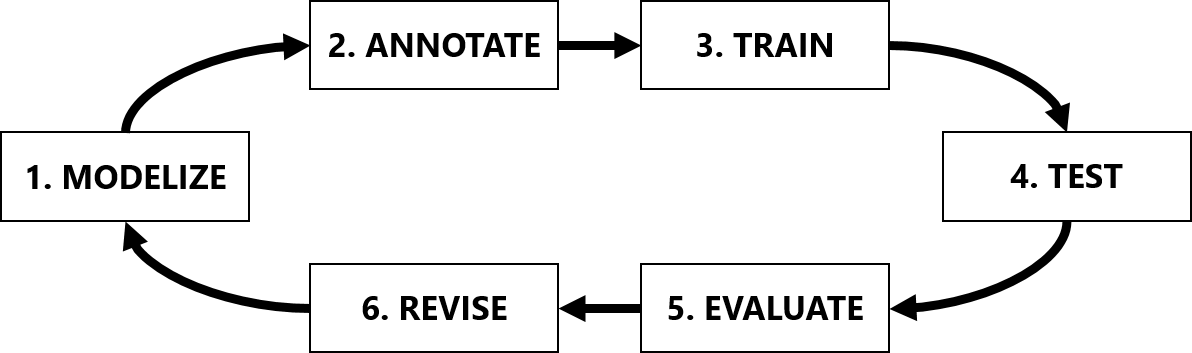
\includegraphics[width=0.95\textwidth]{figures/etatdelart-pustejovsky-2012-cycle-matter}
				\caption{
					Cycle \texttt{MATTER} structurant un projet d'annotation en six étapes principales: \textit{\textbf{M}odelize}, \textit{\textbf{A}nnotate}, \textit{\textbf{T}rain}, \textit{\textbf{T}est}, \textit{\textbf{E}valuate} et \textit{\textbf{R}evise}.
				}
				\label{figure:2.2.1-ORGANISATION-ANNOTATION-ETAPES-CLES-MATTER}
			\end{figure}
			
			% Collecte
			% M, A, mais aussi MAMA
			% TT, mais aussi Train Dev Test, puis Evaluate
			% Revise
			
			% Step 1: Modelisation
			\paragraph{1. « Modelize ».}
				\todo[inline]{SECTION: À RÉDIGER}
			
			% Step 2: Annotate
			\paragraph{2. « Annotate ».}
				\todo[inline]{SECTION: À RÉDIGER}
			
			% Step 3: Train
			\paragraph{3. « Train ».}
				\todo[inline]{SECTION: À RÉDIGER}
			
			% Step 4: Test
			\paragraph{4. « Test ».}
				\todo[inline]{SECTION: À RÉDIGER}
			
			% Step 5: Evaluate
			\paragraph{5. « Evaluate ».}
				\todo[inline]{SECTION: À RÉDIGER}
			
			% Step 6: Revise
			\paragraph{6. « Revise ».}
				\todo[inline]{SECTION: À RÉDIGER}
		
		
		%%%
		%%% Subsection 2.2.2: Portraits des acteurs intervenant sur un projet d'annotation.
		%%%
		\subsection{Portraits des acteurs intervenant sur un projet d'annotation}
		\label{section:2.2.2-ORGANISATION-ANNOTATION-ACTEURS}
			\todo[inline]{SECTION: À RÉDIGER: \\
				- Acteurs: Objectifs, Rôles, Compétences, ... ; \\
				~~~~ - Axe métier (business expert) ; \\
				~~~~ - Axe technique (data scientist) ; \\
				~~~~ - Axe manipulation (data analyst) ; \\
				~~~~ - Axe projet (project leader) ;
			}
		
		
		%%%
		%%% Subsection 2.2.3: Exemples de logiciels utilisés pour annoter.
		%%%
		\subsection{Exemples de logiciels utilisés pour annoter}
		\label{section:2.2.3-ORGANISATION-ANNOTATION-LOGICIELS}
			\todo[inline]{SECTION: À RÉDIGER: \\
				- Outils: Liste, Avantages, Inconvénients, Fonctionnalités ;
				~~~~ - Excel
				~~~~ - prodigy
					% - Glozz [Widlöcher & Mathet, 2009] http://www.glozz.org/
					% - Callisto [Day et al., 2004]
					% - MMAX2 [Müller, 2006] https://github.com/ottiram/MMAX2
					% - PALinkA [Orăsan, 2003]
					% - Gate [Cunningham_2022] https://gate.ac.uk/
					% - Brat [Stenetorp et al., 2012] http://brat.nlplab.org/
					% - WebAnno [Yimam et al., 2013] https://webanno.github.io/webanno/
					% - Inception [Klie et al., 2018] https://inception-project.github.io/
			}
		
		
		% Conclusion.
		\begin{leftBarSummary}
			\begin{todolist}
				\item[\itemok] Un projet d'annotation s'organise généralement en cycle (\texttt{MATTER}) au cours duquel l'annotateur créé une représentation mentale des données, réalise son annotation, entraîne son modèle, puis révise sa représentation mentale des données en fonction des performances du modèle obtenu.
				\item[\itemok] Un tel projet d'annotation nécessite une diversité de connaissances et de compétences (\textit{connaissances métiers, connaissances techniques, maîtrise de l'apprentissage automatique, ...}), faisant ainsi collaborer un grand nombre d'acteurs qualifiés pour une ou plusieurs phase du cycle d'annotation.
			\end{todolist}
		\end{leftBarSummary}
	
	
    %%%%%--------------------------------------------------------------------
    %%%%% Section 2.3: Les nombreux défis de l'annotation
    %%%%%--------------------------------------------------------------------
    \section{Les nombreux défis de l'annotation}
	\label{section:2.3-DEFIS-ANNOTATION}
		\todo[inline]{SECTION: TITRE À TROUVER: "\textit{Défis annotation}"}
		\todo[inline]{SECTION: À RÉDIGER: \\
			- Les données doivent être représentatives (Qualité, Biais, Equilibrage, ...) ; \\
			- Donc la tâche est complexe (...) ; \\
			- Donc les opérateurs régulent leur charge de travail () !
		}
		
		
		%%%
		%%% Subsection 2.3.1: Défis concernant le besoin de qualité des données.
		%%%
		\subsection{Défis concernant le problème de qualité des données}
		\label{section:2.3.1-DEFIS-ANNOTATION-ASPECT-DONNEES}
			\todo[inline]{SECTION: TITRE À TROUVER: "\textit{Données de qualité}"}
			\todo[inline]{SECTION: À RÉDIGER}
		
		
		%%%
		%%% Subsection 2.3.2: Défis concernant la complexité inhérente à la tâche d'annotation.
		%%%
		\subsection{Défis concernant la complexité inhérente à la tâche d'annotation}
		\label{section:2.3.2-DEFIS-ANNOTATION-ASPECT-COMPLEXITE}
			\todo[inline]{SECTION: TITRE À TROUVER: "\textit{Tache complexe}"}
			\todo[inline]{SECTION: À RÉDIGER}
		
		
		%%%
		%%% Subsection 2.3.3: Défis concernant les différences de comportements intra- et inter-annotateurs.
		%%%
		\subsection{Défis concernant les différences de comportements intra- et inter-annotateurs}
		\label{section:2.3.3-DEFIS-ANNOTATION-ASPECT-HUMAIN}
			\todo[inline]{SECTION: TITRE À TROUVER: "\textit{Régulation de la charge de travail}"}
			\todo[inline]{SECTION: À RÉDIGER}
		
		
		% Conclusion.
		\begin{leftBarSummary}
			\begin{todolist}
				\item[\itemok] L'enjeu d'un projet d'annotation consiste à avoir des données de qualité qui soient représentatives du problème à traiter ;
				\item[\itemok] Or la tâche d'annotation et son exigence de qualité engendre de la complexité, et donc une charge de travail élevée ;
				\item[\itemok] Pour réguler cette charge de travail élevée, chaque opérateur va adapter sa tâche pour la rendre supportable, créant ainsi des différences de comportement.
			\end{todolist}
		\end{leftBarSummary}
	
	
    %%%%%--------------------------------------------------------------------
    %%%%% Section 2.4:
    %%%%%--------------------------------------------------------------------
    \section{Techniques et organisations avancées d'annotation}
	\label{section:2.4-AVANCEES-ANNOTATION}
		\todo[inline]{SECTION: TITRE À TROUVER: "\textit{Techniques avancées d'annotation}"}
		\todo[inline]{SECTION: À RÉDIGER: \\
			- Sur les données: ... \\
			- Sur la complexité: ... \\
			- Sur les annotateurs: ...
		}
		
		
		%%%
		%%% Subsection 2.4.1: Avancées concernant le besoin de qualité des données.
		%%%
		\subsection{Avancées concernant le besoin de qualité des données}
		\label{section:2.4.1-AVANCEES-ANNOTATION-ASPECT-DONNEES}
			\todo[inline]{SECTION: TITRE À TROUVER: "\textit{Données de qualité}"}
			\todo[inline]{SECTION: À RÉDIGER}
		
		
		%%%
		%%% Subsection 2.4.2: Avancées cla diminution de la complexité de la tâche d'annotation
		%%%
		\subsection{Avancées concernant la diminution de la complexité de la tâche d'annotation}
		\label{section:2.4.2-AVANCEES-ANNOTATION-ASPECT-COMPLEXITE}
			\todo[inline]{SECTION: TITRE À TROUVER: "\textit{Tache complexe}"}
			\todo[inline]{SECTION: À RÉDIGER}
		
		
		%%%
		%%% Subsection 2.4.3: Concernant la réduction des différences de comportements intra- et inter-annotateurs.
		%%%
		\subsection{Avancées concernant la réduction des différences de comportements intra- et inter-annotateurs}
		\label{section:2.4.3-AVANCEES-ANNOTATION-ASPECT-HUMAIN}
			\todo[inline]{SECTION: TITRE À TROUVER: "\textit{Régulation de la charge de travail}"}
			\todo[inline]{SECTION: À RÉDIGER}
		
		
		% Conclusion.
		\begin{leftBarSummary}
			\begin{todolist}
				\item[\itemok] (TODO)
			\end{todolist}
		\end{leftBarSummary}

    %%%%%--------------------------------------------------------------------
    %%%%% Section 2.5:
    %%%%%--------------------------------------------------------------------
    \section{(\textit{conception toujours difficile en entreprise})}
	\label{section:2.5-RETOUR-EXPERIENCES-INDUSTRIELLES}
		\todo[inline]{SECTION: TITRE À TROUVER: "\textit{REX entreprise}"}
		\todo[inline]{SECTION: À RÉDIGER: \\
			- Modélisation toujours compliquée ; \\
			- Expert métier "pas à leur place" ; \\
			- Peu de stratégies de notre revue mises en oeuvre...
		}